

\section{A first look at linear equations}

Your sink, I'm sorry to say, is clogged.  The bottle of drain opener didn't clear it out and you're expecting dinner guests in a few hours.  Your brother-in-law has offered to help, but last time he tried he only made it worse.  The plumber will charge you \$100 just to come to your house.  In addition, there will be a charge of \$75 per hour for the service.  If you decide to call the plumber, what will it cost?

What will it cost if the plumber takes 1 hour, 2 hours, or 3 hours?  If the plumber takes one hour, then he'll charge you \$100 for showing up and \$75 for the one hour of work.  So, the total plumber's bill will be 
$$100 + 75 = \$175$$  
For two hours, there's still the \$100 charge, but also \$75 for each of the two hours.  That's an additional charge of 
$$2 \text{ hours} \ast \frac{\$75}{\text{hour}} =2 \times 75= \$150$$  
So, the total plumber's bill will be 
$$\$100 + \$150 = \$250$$
Try this calculation all at once.
$$\$100 + 2 \text{ hours} \ast \frac{\$75}{\text{hour}} = 100 + 2 \times 75 = \$250$$   
Let's hope it wouldn't take the plumber as long as three hours, but if it did, we can do a similar calculation.  Add the fixed charge of \$100 to the additional charge of \$75 for each of the three hours.  The plumber's bill would be 
$$ \$100 + 3 \text{ hours} \ast \frac{\$75}{\text{hour}} = 100 + 3 \times 75 = \$325$$  

What would it cost if the plumber takes only $\frac{1}{2}$ hour?  The plumber's bill would be 
$$\$100 + \frac{1}{2} \text{ hours} \ast \frac{\$75}{\text{hour}} =100 + .5 \times 75  = \$100 + \$37.50 = \$137.50$$  
Notice we used $\frac{1}{2}=1 \div 2 = .5$, bet you knew that.

What would happen if the plumber was taking so long that before he got there you dumped another bottle of drain opener in the sink and that did the trick.  But before you could call and cancel the plumber, wouldn't you know it, there he was.  What do you owe him for that 0 hours of work?  Probably \$100.  Unless your plumber is super sympathetic and tells you to ``forget it.''  %So, when $T=0$ the bill is $P=100$.

The plumber's charge will depend on the amount of time it takes to unclog the sink.  We can name these variables.
\begin{center}
\begin{tabular} {l} 
$T=$ time plumber takes (hours) $\sim$ indep \\
$P= $ total plumber's charge (\$) $\sim$ dep \\ 
\end{tabular}
\end{center}

Look at the the relationship between $T$ and $P$ by making a table to describe how the plumber's bill is a function of the time.
\begin{center}
\begin{tabular} {|c| |c |c |c |c |c |c |} \hline
$T$ & 0 & .5 & 1 & 2 & 3 \\ \hline
$P$ & 100 & 137.50 & 175 & 250 & 325 \\ \hline
\end{tabular}
\end{center}

Each time we knew how long the plumber spent and calculated the plumber's bill $P$ by starting with the trip charge of \$100 and adding in \$75 times the number of hours.  For example, for 3 hours we calculated
$$ \$100 + 3 \text{ hours} \ast \frac{\$75}{\text{hour}} = \$325$$
We have a name for the number of hours in general; it is $T$.  So for $T$ hours, we would calculate
 $$\$100 + T \text{ hours} \ast \frac{\$75}{\text{hour}}=P $$  
 See how we just put the $P$ in for \$325 and $T$ where the 3 hours was?  We're just generalizing from our example.  Drop the units and we have our equation.  If the plumber works for $T$ hours, then the cost is \$$P$ where 
 $$P = 100 + T \ast 75$$  
 We started the equation ``$P=$'' because it is a convention to begin equations with the dependent variable, when possible.
 
 An \textbf{equation} is a formula that shows how the value of the dependent variable (like $P$) depends on the value of the independent variable (like $T$).  Usually an equation is in the form dependent variable equals a formula involving the independent variable.  We remember this template as
 \begin{center}
\textbf{Equation:} \quad dep= formula involving indep
 \end{center}
An equation is another way to describe a function.  It carries a lot of information in only a few symbols.

There is a mathematical convention that we write numbers before letters in an equation. So, instead of $T \ast 75$ we should write $75 \ast T$.  There's a conventional shorthand for this product:  when a number and letter are next to each other, it means that they are multiplied.  So, instead of $75 * T$ we should write $75T$. Thus our equation is normally written as $$P = 100 + 75T.$$  You'll have to remember the hidden multiplication when you're calculating.  

If you wanted to write the equation as $$P = 75T + 100,$$ that would be okay too.  We can add the \$100 trip charge first, like we did in our examples, or at the end.  Same answer.

Suppose the plumber shows up at your house and fixed the sink in 25 minutes.  Whew!  No sooner do you pay your bill than your first dinner guest arrives.  How much do you owe the plumber?  Notice that 
$$25 \text{ minutes} \ast \frac{1 \text{ hour}}{60 \text{ minutes}} = 25 \div 60 = .4166\ldots \text{ hours}$$  
Therefore for 25 minutes we have $T \approx .4166$  
Using our equation we get $$ P = 100 + 75\ast .4166 = 100 + 75 \times \underline{.4166} = 131.245 \approx \$131.25.$$  It was important that we rounded off our final answer because we had rounded off to get .4166 along the way.  We could have done the entire calculation at once (avoiding the round off error) as 
$$100 + 75 \times 25 \div 60 =131.25$$
Either way, we owe the plumber \$131.25.

% SU do you need to talk a bit about how you found the scale for this graph?

If we plot the points from the table of values in a graph, we see that the points lie on a line.  
\begin{center}
\scalebox {1} {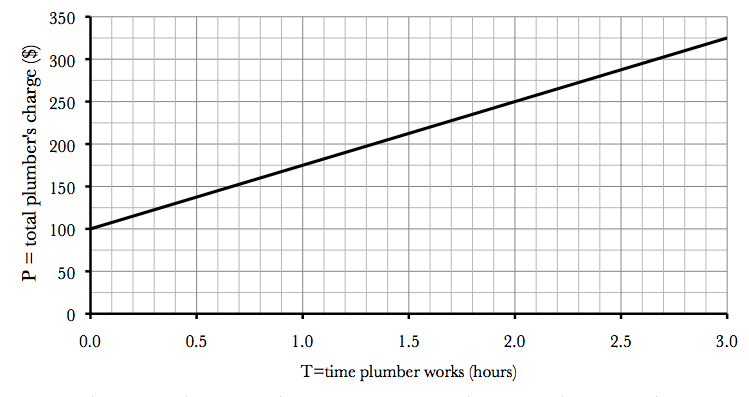
\includegraphics [width = 6in] {Plumber.png}}
\end{center}
Why is the graph a line?  Remember that the rate of change tells us how steep the graph is.  For example, let's find the rate of change between 1 hour and 2 hours.
$$\text{rate of change} = \frac{\text{change dep}}{\text{change indep}} = \frac{\$250 - \$175}{2 \text{ hours} - 1 \text{ hour}} = \frac{\$75}{1 \text{ hour}} = \$75 \text{ per hour}$$  
Sure!  We knew that.  The plumber charges an extra \$75 for each extra hour he works.  The rate of change is precisely \$75/hour, no matter where we calculate it.  Since the rate of change is constant, the graph is the same steepness everywhere.  So, the graph is a line, and the function is \textbf{linear}.  Another way to say this is a function with constant rate of change is \textbf{linear}.  The plumber's total charge is a linear function of time.

Look back at our equation.  $$P = 100 + 75T$$  Any linear equation fits this template. 

\bigskip
 \framebox{
 \begin{minipage}[c]{.85\textwidth}  
~ \bigskip \\  \textsc{Linear equation template:} \quad dep = start + slope $\ast$ indep\\ ~ \bigskip
\end{minipage}
}
\bigskip

Notice our two variables are in our equation and there are two constants. Each constant has its own meaning.  The first constant is 100 and it is measured in dollars.  It is the trip charge, the fixed amount we would owe the plumber even if he does 0 hours work.  In our standard form we refer to this quantity as the \textbf{starting value} (or \textbf{start} for short), but it's official name is \textbf{intercept}.  On the graph it's where the line crosses the vertical axis.  Think of a football player (running along the vertical axis) intercepting a pass (coming in the line).  We can find the intercept from our equation by plugging in $T = 0$ so that $$P = 100 + 75 \times 0 = 100$$

The second constant is 75 and though its tempting to say it is measured in dollars, it is really measured in \$ per hour.  This number is the rate of change and in the context of linear equations it gets its own name too.  Its called the \textbf{slope}.  Since the rate of change measures the steepness of any curve or line, the word ``slope'', like mountain slope, makes sense.  In our plumber example the intercept was \$100 and the slope was \$75/hour.  

%\newpage

%%\section{A first look at linear equations}

\begin{center}
\line(1,0){300} %\line(1,0){250}
\end{center}

\section*{Homework}

\noindent \textbf{Start by doing Practice exercises \#1-4 in the workbook.}

\bigskip

\noindent \textbf{Do you know \ldots}

\begin{itemize} 
\item How to generalize from an example to find an equation? 
\item Where the dependent variable usually is in an equation? 
\item What the slope of a linear function means in the story and what it tells us about the graph? 
\item What the intercept of a linear function means in the story and what it tells us about the graph?  
\item The template for a linear equation? \emph{Ask your instructor if you need to remember the template or if it will be provided during the exam.} 
\item Where the slope and intercept appear in the template for a linear equation?  
\item What makes a function linear? 
\item How to plot negative numbers on a graph? 
\item What the graph of a linear function looks like? 
 \item[~] \textbf{If you're not sure, work the rest of exercises and then return to these questions.  Or, ask your instructor or a classmate for help.} 
\end{itemize}

\subsection*{Exercises}

\begin{enumerate} 
\setcounter{enumi}{4}

\item Plumbers are really expensive, so I'm comparing their rates.  Write an equation for each possibility, using the same variables as our example:  $T$ for the time the plumber takes (in hours) and $P$ for the plumber's total charge (in dollars). 

 \hfill \emph{Story also appears in 4.1 \#4}
\begin{enumerate}
\item James charges \$50 to show up plus \$120 per hour. 
\item Jo the plumber is just getting started in the business.  She charges \$45 to show up plus \$55 per hour.
\item Mario advertises ``no trip charge'' but his hourly rate is \$90 per hour. 
\item Not to be outdone, Luigi offers to unclog any drain for \$150, no matter how long it takes.  (``Wake up, Luigi! The only time plumbers sleep on the job is when we're working by the hour,'' says Mario.)
\end{enumerate} 

\item Abduwali has just opened a restaurant. He spent \$82,500 to get started but hopes to earn back \$6,300 each month.  \hfill \emph{Story also appears in 3.1 Exercises}
\begin{enumerate}
\item If all goes according to plan, will he have made money 10 months from now?
\item Name the variables and write an equation relating them.
\item Identify the slope and intercept, along with their units, and explain what each means in terms of the story. 
\item Make a small tables of values and use it to draw a graph showing Abduwali's profit.
\end{enumerate}

\item When Gretchen walks on her treadmill, she burns 125 calories per mile.

\hfill \emph{Story also appears in 3.1 and 3.2 Exercises}
\begin{enumerate}
\item How many calories will Gretchen burn if she walks 2.3 miles?
\item Name the variables and write an equation relating them.
\item Identify the slope and intercept, along with their units, and explain what each means in terms of the story. 
\item Make a table showing the calories she burns walking 0, 1, 2, 3, or 4 miles.
\end{enumerate} 

\item The local burger restaurant had a promotion this summer.  Typically a bacon double cheeseburger costs \$7.16.  They reduced the price by 2\textcent~for each degree in the daily high temperature. For example, if the high temperature was 80$^\circ$F, they would decrease the price by $0.02 \times 80 = \$1.60$, so the double cheeseburger would cost $7.16-1.60=\$5.56$.  Mmmm.
\hfill \emph{Story also appears in 3.1 \#4} 
\begin{enumerate}
\item Name the variables in the story and write a linear equation relating them.
\item Is the function increasing or decreasing?
\item Make a table showing the price of a bacon cheeseburger when the daily high temperature is 65$^\circ$F, 75$^\circ$F, and 90$^\circ$F.
\item Draw a graph illustrating how the price of a bacon double cheeseburger depends on the temperature.  Start the temperature on your graph at 60$^\circ$F.
\end{enumerate} 

\item A report on health care back in 1975 stated that the U.S. had around 1,466,000 hospital beds and since then the number of beds has declined by around 16,000 beds  per year.   
\hfill \begin{footnotesize} Source:  Center for Disease Control and Prevention \end{footnotesize}
\begin{enumerate}
\item Name the variables, including units and dependence.
\item Write an equation illustrating the function.
\item Is the function increasing or decreasing?
\item Make a table showing the number of hospital beds projected for 1980, 1990, 2000, 2010, and 2020.  
\item  At this rate of decline, in what year will we have only \nicefrac{1}{2} million beds?  First estimate the answer from your table.  Then figure it out, to the nearest year.
\end{enumerate}
%FROM:  http://www.cdc.gov/nchs/data/hus/2010/113.pdf
% 1975 = 1,465,828 then 1980 = 1,364,516 then 1990=1,213,327
% then 1995=1,080,601 then 2000=983,628 then 2007=845,199 then 2008=951,045
% FROM:

\item The stretch of interstate highway through downtown averages 1,450 cars per hour during the morning rush hour.  The economy is improving (finally), but with that the county manager predicts traffic levels with increase around 130 cars per hour more each week for the next couple of years. \hfill \emph{Story also appears in 3.1 Exercises}
\begin{enumerate}
\item Name the variables and write an equation relating them.
\item Make a table showing the number of cars per hour anticipated now and in 2 years, 4 years, 6 years, 8 years, and 10 years.
\item Significant slowdown are expected if traffic levels exceed 2,000 cars per hour.  When do they expect that will happen? Estimate your answer from your table.  (Or, figure it out.)
\item If traffic levels exceed 2,500 the county plans to install control lights at the on ramps.  When is that expected to happen?   
\end{enumerate} 

\end{enumerate}

